\section{Auswertung}
\label{sec:Auswertung}


In Tabelle \ref{tab:tabelle1} ist der experimentell bestimmte Wert $U_out$ abhängig von $\increment \varphi$ aufgelistet.
Zudem wird ein, mit Gleichung \ref{eqn:cos} berechneter theoretischer Wert, in die Tabelle eingetragen.
Zudem wird die Abweichung $A_{e,t}$ vom theoretischen Wert mit 
\begin{equation}
  A_{n,m}=\Biggl|\frac{U_{n}-U_{m}}{U_{m}}\Biggr|
  \label{eqn:Abweichung}
\end{equation}
berechnet.
Außerdem wurden die Messung mit einem Rauschsignal ebenfalls in die Tabelle eingetragen.
Hier wurde mit Formel \ref{eqn:Abweichung} die Abweichung $A_{N,e}$vom Wert mit Rauschen zu dem ohne gebildet.


\begin{table}
  \centering
  \caption{Aufgelistet ist die gemessene Ausgangsspannung abhängig von Phasenverschiebung der Referenzspannung. 
  Zudem ist ein theoretischer Wert, sowie die Abweichung zu diesem, eingetragen.
  Außerdem wurden die Werte, die bei einem Rauschen gemessen wurden, eingetragen und die Abweichung zu den Werten ohne Rauschen bestimmt.
  }
  \label{tab:tabelle}
  \sisetup{table-format=1.1, per-mode=reciprocal}
  \begin{tblr}{
      colspec = {S[table-format=3.0] S[table-format=1.2] S[table-format=1.2] S[table-foramt=2.2] S[table-format=1.2] S[tanle-format=1.2]},
      row{1} = {guard, mode=math},
      vline{4} = {2}{-}{text=\clap{$\pm$}},
    }
    \toprule
    \varphi \mathbin{/} \unit{\degree} & U_{out} \mathbin{/} \unit{\volt}  & U_{out,t} \mathbin{/} \unit{\volt} & A_{e,t} \mathbin{/} \unit{\percent} & U_{out,N} \mathbin{/} \unit{\volt} & A_{N,e} \mathbin{/} \unit{\percent}\\
    \midrule
    0     &  2.96   &  2.96 &   0.00  &  2.96 &  0.00   \\
    45    &  2.64   &  2.09 &  26.13  &  2.72 &  3.03   \\
    90    &  0.96   &  0.00 &  X      &  0.96 &  0.00   \\
    135   & -1.04   & -2.09 &  50.31  & -1.04 &  0.00   \\
    180   & -2.40   & -2.96 &  18.92  & -2.48 &  3.33   \\
    225   & -2.08   & -2.09 &   6.23  & -2.16 &  3.85   \\
    270   & -0.48   &  0.00 &  X      & -0.48 &  0.00   \\
    315   &  1.60   &  2.09 &  23.56  &  1.52 &  5.00   \\
    360   &  2.96   &  2.96 &   0.00  &  2.96 &  0.00   \\
    \bottomrule
  \end{tblr}
\end{table}


\begin{figure}
  \centering
  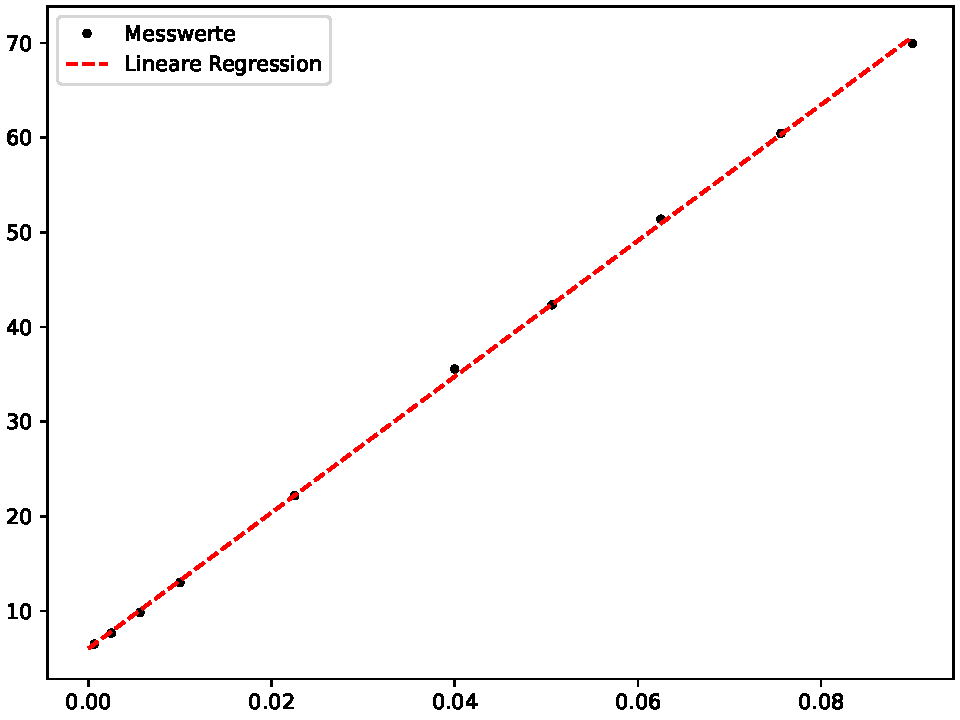
\includegraphics{plot.pdf}
  \caption{Plot.}
  \label{fig:plot}
\end{figure}



